\documentclass[tikz]{standalone}
\usepackage{amsmath}% for \Re and \Im
\def\n{6}
\begin{document}
	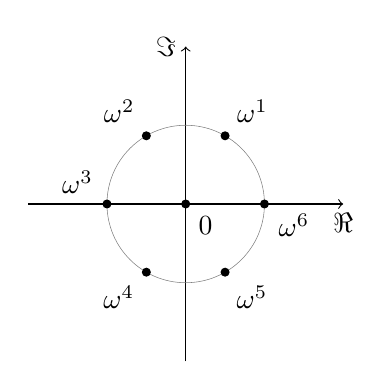
\begin{tikzpicture}[
		dot/.style={draw,fill,circle,inner sep=1pt}
		]
		\draw[->] (-2,0) -- (2,0) node[below] {$\Re$};
		\draw[->] (0,-2) -- (0,2) node[left] {$\Im$};
		\draw[help lines] (0,0) circle (1);
		
		\node[dot,label={below right:$0$}] (O) at (0,0) {};
		\foreach \i in {1,...,\n} {
			\node[dot,label={\i*360/\n-(\i==\n)*45:$\omega^{\i}$}] (w\i) at (\i*360/\n:1) {};
%			\draw[->] (O) -- (w\i);
		}
%		\draw[->] (0:.3) arc (0:360/\n:.3);
%		\node at (360/\n/2:.5) {$\alpha$};
	\end{tikzpicture}
\end{document}